\subsection{Mô hình điều khiển hành vi cho đội hình chữ V}
\label{sec:tra}
Tại mỗi bước thời gian, Robot leader tạo ra cấu trúc ảo hình chữ V bằng cách tạo ra các mục tiêu ảo cho các follower thông qua giao tiếp ngang hàng. Trong phần này, việc điều khiển dựa trên hành vi được đề xuất cho phép các Robot đi theo cấu trúc ảo để duy trì đội hình chữ V trong khi tránh chướng ngại vật và tránh các Robot khác. Hành vi tổng thể do robot thực hiện là sự kết hợp của một số hành vi phụ như là: di chuyển đến mục tiêu, tránh chướng ngại vật, tránh robot và giữ đội hình. Trong các ứng dụng thực tế, mỗi hành vi của robot được nêu dưới dạng véc tơ bao gồm hướng và độ lớn. Trọng số của trong mỗi hành vi có thể thay đổi được bằng cách điều chỉnh tham số. Dựa trên thông tin được phát hiện từ môi trường xung quanh, robot lựa chọn hành vi phù hợp. Từ đó, một di chuyển sẽ được tạo ra. Véc tơ hành vi tổng hợp là tổng của tất cả các véc tơ hành vi cơ bản thiết lập trong robot được định nghĩa là: Hành vi tổng thể của Robot $i$ được tổng hợp bởi một số hành vi phụ khi di chuyển đến mục tiêu $V_{m2g}$, tránh va chạm với vật cản $V_{obs}$ và các Robots khác $V_{adr}$, và giữ đội hình $V_{kf}$ như sau:
\begin{equation}
    V_i=V.f
\label{eq:v}
\end{equation}
Trong đó $V=[V_{m2g}$, $V_{ath}$, $V_{adr}$, $V_{kf}]$ là hành vi phụ, và $f=[f_{m2g}$, $f_{ath}$, $f_{adr}$, $f_{kf}]^T$ là tham số điều khiển. Với $P_i=[x_i, y_i,z_i]^T$ là vị trí của Robot thứ i. Các hành vi phụ được thể hiện như sau:

\subsubsection{Hành vi di chuyển đến đích}
\begin{figure}[h]
    \centering
    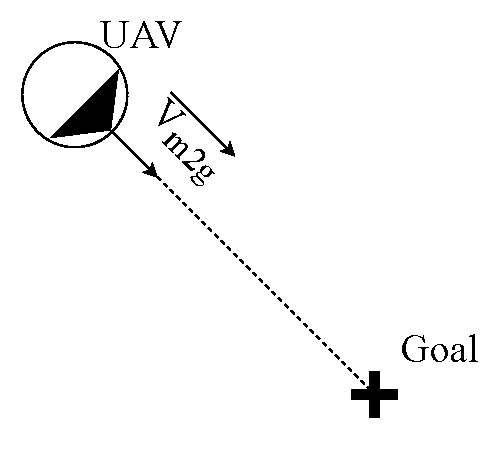
\includegraphics[width = 0.3\textwidth]{chapter3/image/Behavior_m2g_cropped.pdf}
    \caption{Hành vi đi tới đích}
    \label{fig:m2g}
\end{figure}

Hành vi di chuyển đến đích được định hướng bởi Robot leader về phía mục tiêu là một điểm trên đường đi được mô tả trong Hình.\ref{fig:m2g} và được trình bày như sau:
\begin{equation}
    V_{m2g}=\dfrac{1}{d_{m2g}}\left[\begin{array}{c}
    x_{g}-x_i\\
    y_{g}-y_i\\
    z_{g}-z_i
    \end{array}\right]
\end{equation}
Trong đó $P_g=\left[x_g, y_g, z_g\right]^T$ là vị trí đích, và $d_{m2g}$ là khoảng cách giữa Robot leader và mục tiêu.

Tại hành vi này, Robot leader được yêu cầu di chuyển chầm chậm khi những Robot theo sau chưa bắt kịp mục tiêu ảo của chúng. Do đó, tham số điều khiển $f_{m2g}$ được xác định dựa trên lỗi vị trí của các Follower như sau:
\begin{equation}
    f_{m2g}=\left\{\begin{array}{cc}
    a_{m2g} & N_{err}=\emptyset\\
    \dfrac{b_{m2g}}{\max\limits_{i\in N_{err}}\{err_i\}} & N_{err}\neq \emptyset
    \end{array}\right.
\label{eq:m2gp}
\end{equation}
Trong đó $a_{m2g}$ và $b_{m2g}$ là các tham số điều chỉnh; $N_{err}$ là một tập các lỗi vị trí của các Follower với lỗi vị trí lớn hơn một khoảng được xác định trước. Khoảng này có thể được thay đổi định kỳ theo từng bước thời gian thông qua mạng không dây ad-hoc.
 
\subsubsection{Hành vi tránh vật cản}
\begin{figure}[h]
    \centering
    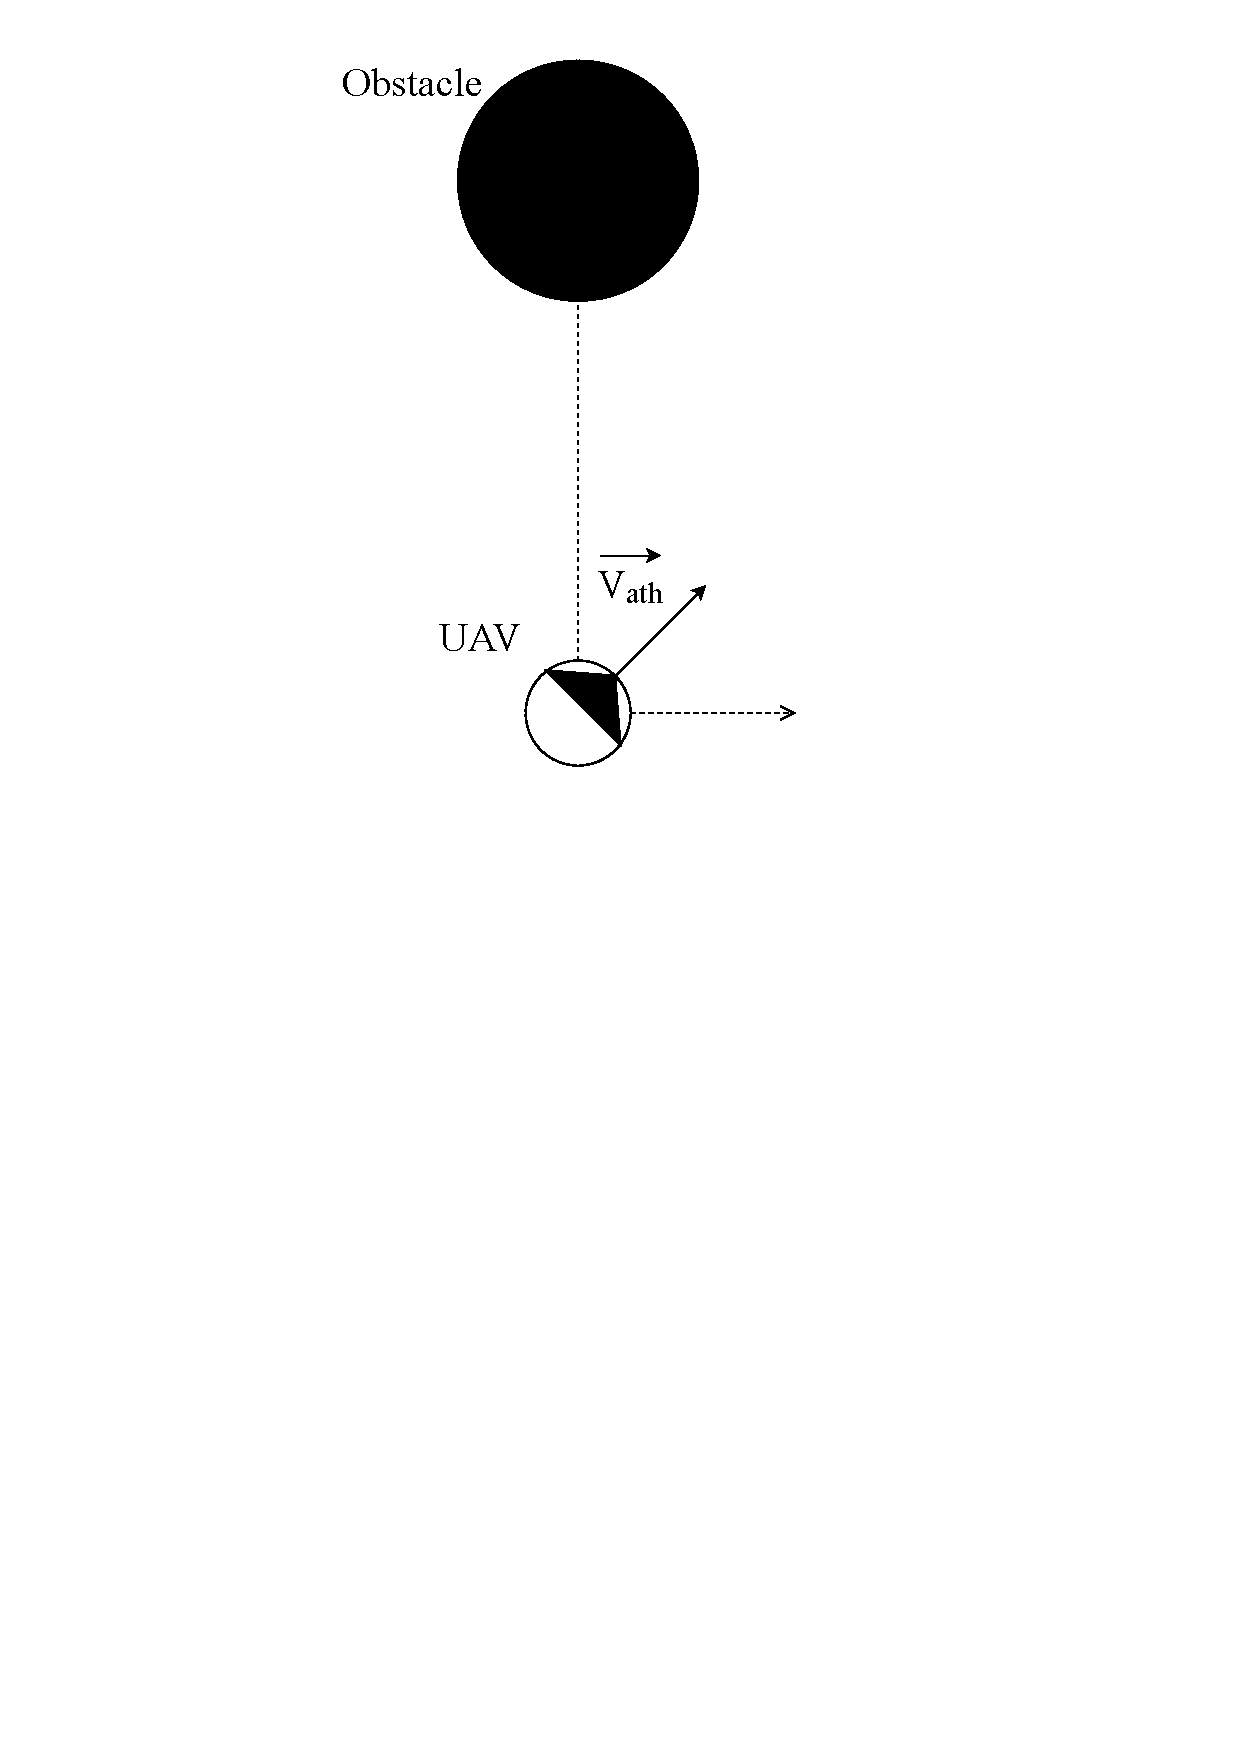
\includegraphics[width = 0.3\textwidth]{chapter3/image/Behavior_obs_cropped.pdf}
    \caption{Di chuyển tránh vật cản}
    \label{fig:bhobs}
\end{figure}

Hành động được thực hiện khi các robot xác định được một vật cản. Cách truyền thống là để một robot di chuyển về phía sau tạo ra một trạng thái cực tiểu cục bộ. Để giải quyết vấn đề này, ta thay đổi hướng chuyển động với một góc 90 độ về phía vật cản. Tại độ cao $z=z_i$, vật cản có thể được mô phỏng như một vòng tròn với vị trí tâm $\left(x_{th},y_{th},z_{th}\right)$ và bán kính $r_{th}$. Do đo, véc tơ tránh vật cản như sau:
\begin{equation}
    \begin{aligned}
        V_{obs}=\frac{1}{d_{ath}^2}
        \left[\begin{array}{c}
        \pm(y_{th}-y_{i})\\
        \mp(x_{th}-x_{i})\\
        z_i
        \end{array}\right]
    \end{aligned}
    \label{eqn:vobs}
\end{equation}

Trong đó $d_{ath}$ là khoảng cách tương đối giữa Robot và vật cản, kí hiệu $\pm$ được xác định bằng việc vật cản ở bên trái hay phải của vị trí mục tiêu. Tham số điều khiển hành vi được xác lập như sau:
\begin{equation}            
    f_{ath}\left(d_{ath}\right)=\left\{ \begin{array}{cc}
    0 & \text{if } d_{ath}\geq b_{ath}\\
    a_{ath}\left(1-\dfrac{d_{ath}}{b_{ath}}\right) & \text{if } d_{ath}<b_{ath}
    \end{array}\right.
\end{equation}
Trong đó $a_{ath}$ và $b_{ath}$ là các tham số điều chỉnh và $d_{ath}$ là khoảng cách giữa robot và vật cản.

\subsubsection{Hành vi tránh va chạm giữa các robot}
\begin{figure}[h]
    \centering
    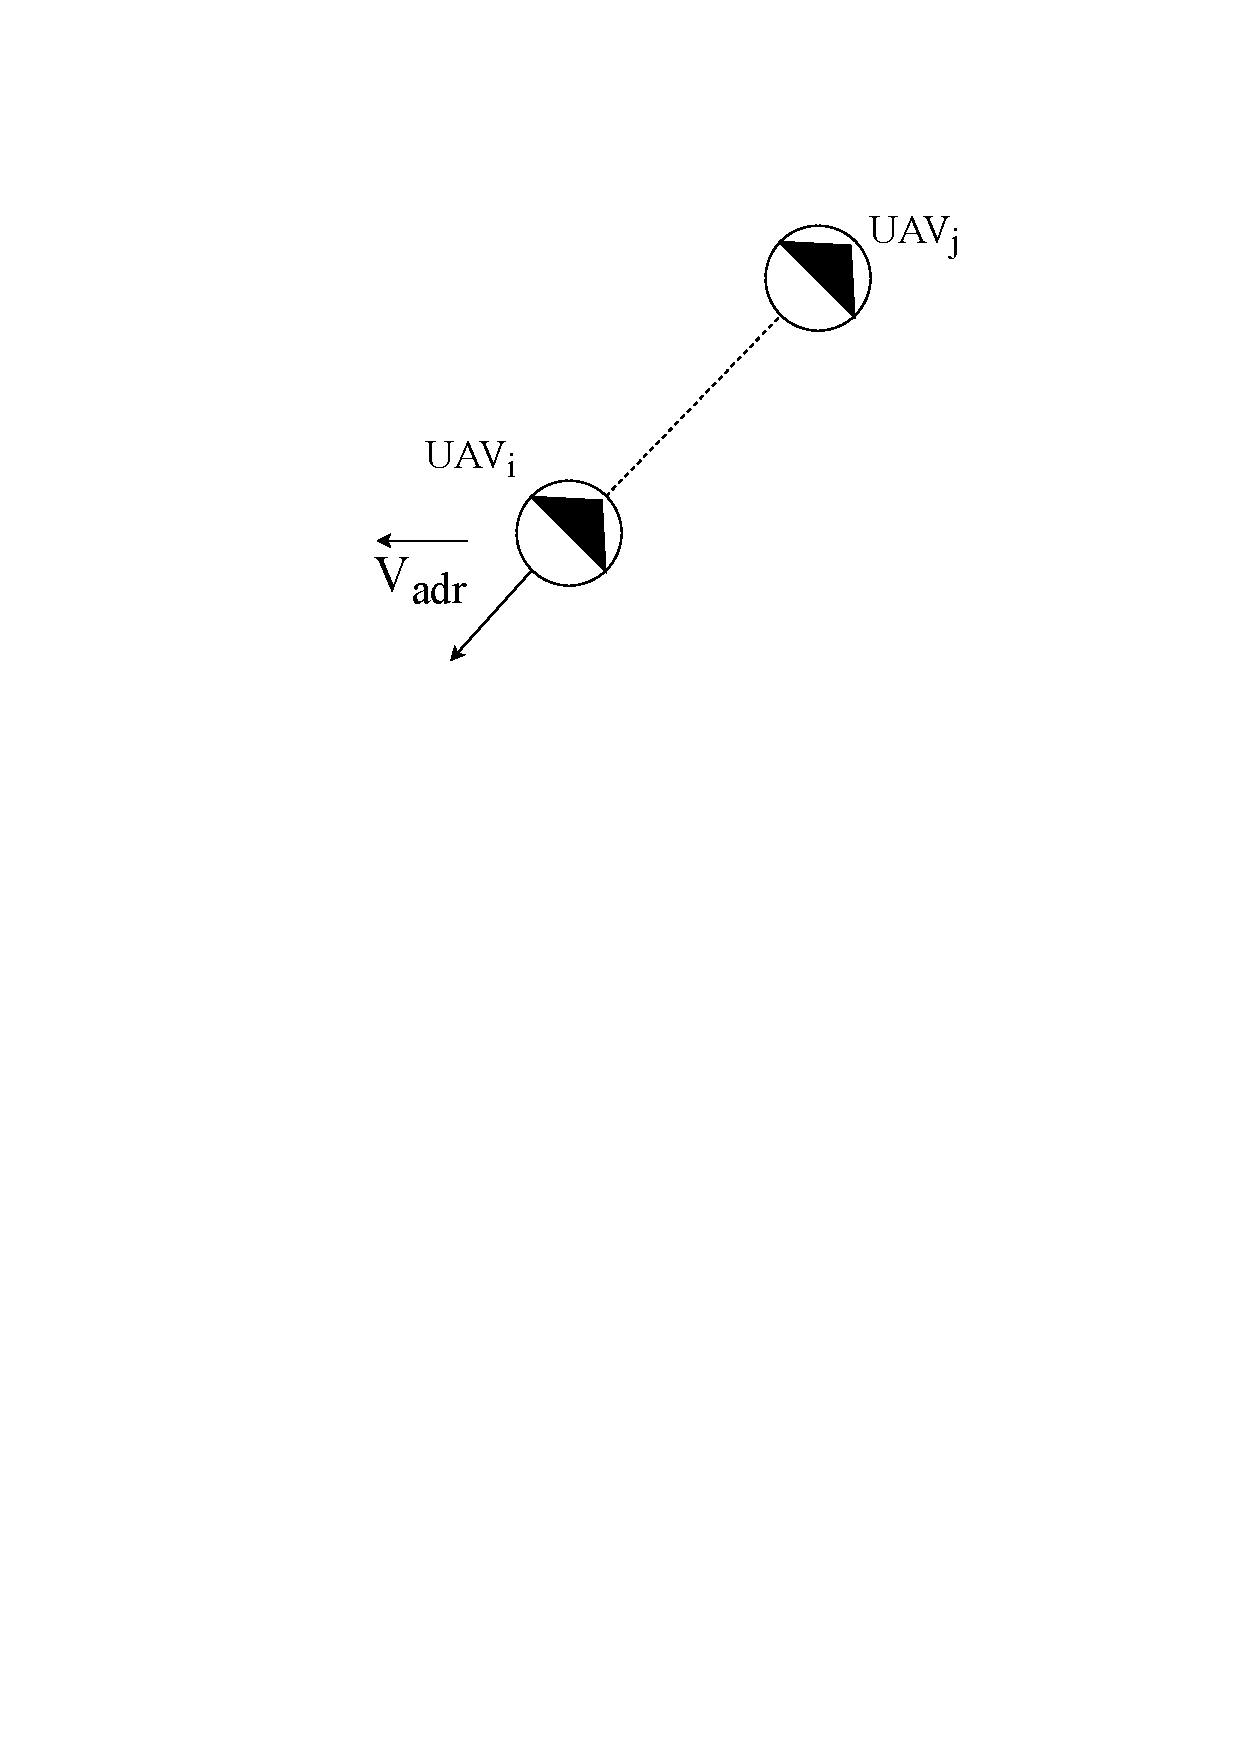
\includegraphics[width = 0.3\textwidth]{chapter3/image/Behavior_AvoidRobot_cropped.pdf}
    \caption{Tránh va chạm với các robot khác}
    \label{fig:adr}
\end{figure}

Hành vi tránh va chạm được kích hoạt khi một Robot quá gần với các Robot khác. Véc tơ tránh va chạm $V_{adr}$ có xu hướng tránh ra khỏi các Robots được xác định như mô tả trong Hình.\ref{fig:adr}, được trình bày như sau:
\begin{equation}
    V_{adr}=\sum_{j=1}^{N_{adr}}\dfrac{1}{d_{adr_{ij}}^2}
    \left[\begin{array}{c}
    x_{dr_j}-x_i\\
    y_{dr_j}-y_i\\
    z_{dr_j}-z_i
    \end{array}\right]
\end{equation}

Trong đó $P_{dr_j}=\left[x_{dr_j},y_{dr_j}, z_{dr_j}\right]^T$ là vị trí của Robot $j$ trong nhóm những Robot được xác định $N_{adr}$, và $d_{adr_{ij}}$ là khoảng cách tương đối giữa Robot $i$ và Robot $j$. Tham số điều khiển của hành vi này được thể hiện như sau:
\begin{equation}
    f_{adr}\left(\overline{d_{adr}}\right)=\left\{ \begin{array}{cc}
    0 & \text{if } \overline{d_{adr}}\geq b_{adr}\\
    a_{adr}\left(1-\dfrac{\overline{d_{adr}}}{b_{adr}}\right) & \text{if } \overline{d_{adr}}<b_{adr}
    \end{array}\right.
\end{equation}
Trong đó $a_{adr}$ và $b_{adr}$ là các tham số điều chỉnh, $\overline{d_{adr}}$ là trung bình của $d_{adr_{ij}}$, $\forall j\in N_{adr}$.

\subsubsection{Hành vi duy trì đội hình}
\begin{figure}[h]
    \centering
    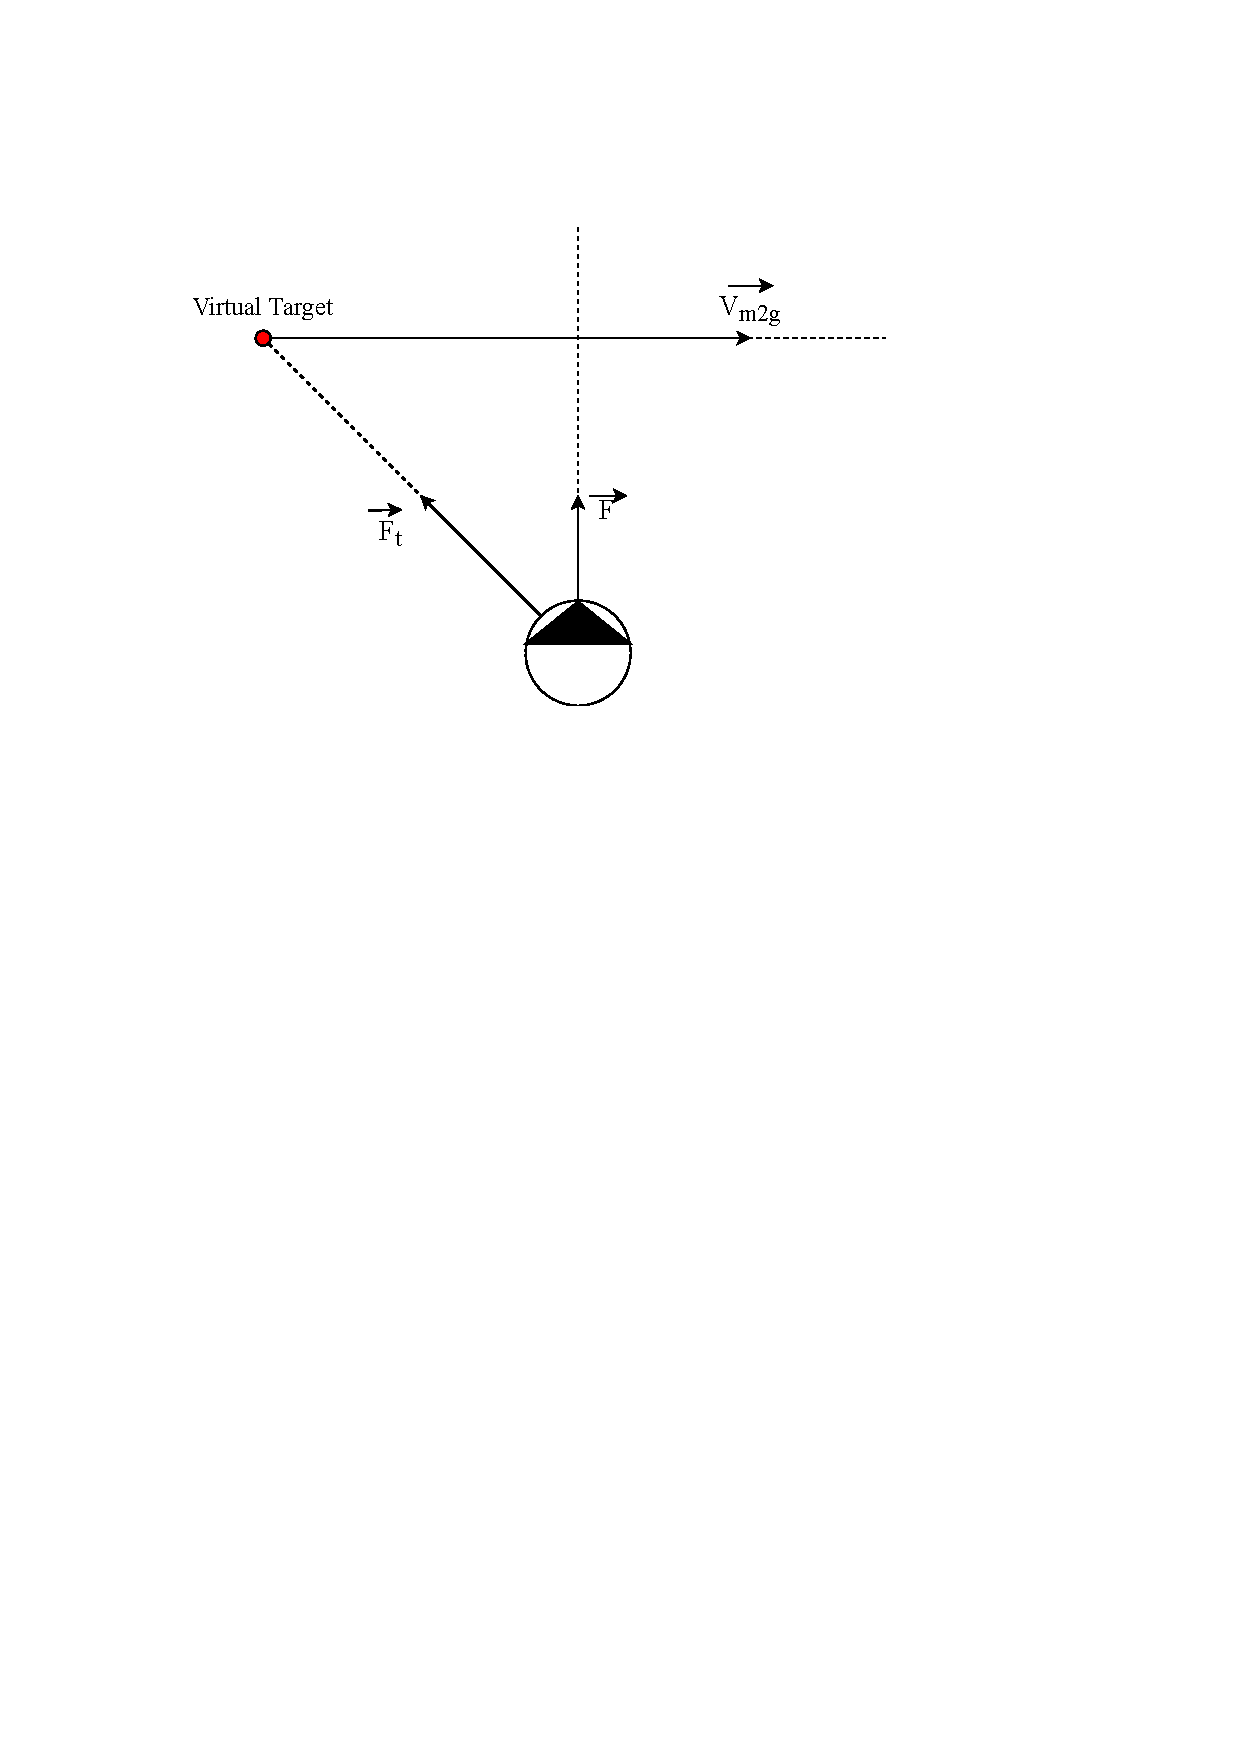
\includegraphics[width = 0.5\textwidth]{chapter3/image/V_Form_Crop.pdf}
    \caption{Giữ đội hình}
    \label{fig:keep}
\end{figure}
Để giữ đội hình luôn trong cấu trúc chữ V cần điều khiển các Robots đi theo cấu trúc chữ V ảo. Phụ thuộc vào vị trí của Robot và mục tiêu của nó trong hướng di chuyển của đội hình, hành vi này có các hành động sau đây:
\begin{itemize}
    \item Mục tiêu ở phía trước Robot: Robot cần đến chỗ mục tiêu, tương tự như hành vi di chuyển đến mục tiêu của Robot leader như mô tả trong hình \ref{fig:m2g}. Do đó, hành vi duy trì đội hình được thể hiện như sau:
         \begin{equation}
            V_{kf}=\dfrac{1}{d_{t}}\left[\begin{array}{c}
            x_{T}-x_i\\
            y_{T}-y_i\\
            z_{T}-z_i\\
            \end{array}\right]
        \end{equation}
        Trong đó $\left[x_T, y_T, z_T\right]^T$ là vị trí mục tiêu, $d_{t}$ là khoảng cách giữa các Robot và các mục tiêu của chúng. Tham số điều khiển $f_{kf}$ được xác định dựa trên khoảng cách $d_{t}$ như sau:
        \begin{equation}
            f_{kf}\left(d_{t}\right)=\left\{ \begin{array}{cc}
            a_{kf} & \text{khi } d_{t}\geq b_{kf}\\
            a_{kf}\dfrac{d_{t}}{b_{kf}} & \text{khi } d_{t}<b_{kf}
            \end{array}\right.
        \end{equation}
        Trong đó $a_{kf}$ và $b_{kf}$ là tham số điều chỉnh.
        
     \item Mục tiêu ở phía sau của Robot: Robot không đi theo mục tiêu vì mục tiêu có xu hướng di chuyển đến gần nó. Do đo, Robot chỉ cần bay chậm theo hướng mục tiêu của đội hình $V_{m2g}$ như Hình.\ref{fig:keep}. Với $F$ là vertor đơn vị giao với hướng mục tiêu $V_{m2g}$, và $F_t$ là véc tơ từ Robot đến mục tiêu của nó. Hành vi duy trì đội hình được xác định như sau:
        \begin{equation}
            V_{kf}= \text{sign}((F\times F_{t}).F)
        \end{equation}
        Tham số điều khiển $f_{kf}$ được định nghĩa như sau:
        \begin{equation}
                 f_{kf}=\frac{a_{kf}}{V_{kf}\times F_t}
            \label{eqn:xyzi1}
        \end{equation}
        Trong đó $\times$ thể hiện phép nhân có hướng.
\end{itemize}